%%%%%%%%%%%%%%%%%%%%%%%%%%%%%%%%%%%%
% Modelo de relatório de Disciplina de MLP a partir da
% classe latex iiufrgs disponivel em http://github.com/schnorr/iiufrgs
%%%%%%%%%%%%%%%%%%%%%%%%%%%%%%%%%%%%
% Definição do tipo / classe de documento e estilo usado
%%%%%%%%%%%%%%%%%%%%
\documentclass[rel-mlp]{iiufrgs}
\usepackage{graphicx}
\graphicspath{ {./images/} }
%%%%%%%%%%%%%%%%%%%%%%%%%%%%%%%%%%%%%%%%%%%%%%%%%%
% Importação de pacotes
%%%%%%%%%%%%%%%%%%%%%%%%%%%%%%%%
% (a A seguir podem ser importados os pacotes necessários para o documento, de acordo 
% com a necessidade)

\usepackage[brazilian]{babel}	    % para texto escrito em pt-br
\usepackage[utf8]{inputenc}         % pacote para acentuação
\usepackage{graphicx}         	    % pacote para importar figuras
\usepackage[T1]{fontenc}            % pacote para conj. de caracteres correto
\usepackage{times}                  % pacote para usar fonte Adobe Times
\usepackage{enumerate}              % para lista de itens com letras
\usepackage{breakcites}
\usepackage{titlesec}
\usepackage{enumitem}
\usepackage{titletoc}               
\usepackage{listings}			    % para listagens de código-fonte
\usepackage{mathptmx}               % p/ usar fonte Adobe Times nas formulas matematicas
\usepackage{url}                    % para formatar URLs
\usepackage{color}				    % para imagens e outras coisas coloridas
%\usepackage{fixltx2e}              % para subscript
%\usepackage{amsmath}               % para \epsilon e matemática
%\usepackage{amsfonts}
%\usepackage{setspace}			    % para mudar espaçamento dos parágrafos
%\usepackage[table,xcdraw]{xcolor}  % para tabelas coloridas
%\usepackage{longtable}             % para tabelas compridas (mais de uma página)
%\usepackage{float}
%\usepackage{booktabs}
%\usepackage{tabularx}
%\usepackage[breaklinks]{hyperref}
\usepackage{longtable}

\usepackage[alf,abnt-emphasize=bf]{abntex2cite}	% pacote para usar citações abnt

%%%%%%%%%%%%%%%%%%%%%%%%%%%%%%
% Macros, ajustes e definições
%%%%%%%%%%%%%%%%%%%%%%%%%%%%%%%

% define estilo de parágrafo para citação longa direta:
\newenvironment{citacao}{
    %\singlespacing
    %\footnotesize
    \small
    \begin{list}{}{
        \setlength{\leftmargin}{4.0cm}
        \setstretch{1}
        \setlength{\topsep}{1.2cm}
        \setlength{\listparindent}{\parindent}
    }
    \item[]}{\end{list}
}

\usepackage{beramono}
\usepackage{xcolor}

% adiciona a fonte em figuras e tabelas
\newcommand{\fonte}[1]{\\Fonte: {#1}}

% Ative o seguinte caso alguma nota de rodapé fique muito longa e quebre entre múltiplas
% páginas
%\interfootnotelinepenalty=10000

% Informações gerais                                  
% título
\title{Relatório Final - Grupo Destemidos - Jogo Frogger em Linguagem Scala}

% autor
\author{Varriale Damian}{Giovanna}
\author{Saraiva Millani}{Lorenzo}
\author{Jose kunz Filho}{Mario}

% Professor orientador da disciplina
\advisor[Prof.~Dr.]{Mello Schnorr}{Lucas}

% Nome do(s) curso(s):
\course{Curso de Graduação em Ciência da Computa{\c{c}}{\~a}o e Engenharia de Computação}

% local da realização do trabalho 
\location{Porto Alegre}{RS} 
% data da entrega do trabalho (mês e ano)
\date{11}{2018}

% Palavras chave
\keyword{Programação}
\keyword{Scala}
\keyword{Frogger}

%%%%%%%%%%%%%%%%%%%%%%%%%%%%%%%%%%%%%%%%%%%%%%%
% Início do documento e elementos pré-textuais
%%%%%%%%%%%%%%%%%%%%%%%%%%%%%%%%%%%%%%%%%%%%%%%
% Declara início do documento
\begin{document}

\lstdefinestyle{myScala}{
  frame = none,
  language = Scala,
  aboveskip = 3mm,
  belowskip = 3mm,
  showstringspaces = false,
  columns = flexible,
  basicstyle = {\small\ttfamily},
  numbers = none,
  numberstyle = \color{gray},
  keywordstyle = \color{blue},
  commentstyle = \color{green},
  stringstyle = \color{magenta},
  frame = single,
  breaklines = true,
  breakatwhitespace = true,
  tabsize = 3,
}

\lstdefinestyle{myJava}{
  frame=none,
  language = Java,
  aboveskip=3mm,
  belowskip=3mm,
  showstringspaces=false,
  columns=flexible,
  basicstyle={\small\ttfamily},
  numbers=none,
  numberstyle = \color{gray},
  keywordstyle = \color{green},
  commentstyle = \color{blue},
  stringstyle = \color{magenta},
  frame=single,
  breaklines=true,
  breakatwhitespace=true,
  tabsize=3,
}

\lstset{style = myScala} %daqui pra baixo os codigos estarão em estilo scala
%% usar o mesmo comando mas com \lstset{style = myJava} antes do \begin pra ter o estilo Java

% inclui folha de rosto 
\maketitle      

\selectlanguage{brazilian}

% Sumario
\tableofcontents

%%%%%%%%%%%%%%%%%%%%%%%%%%%%%%%%%%%%%%%
% Aqui comeca o texto propriamente dito
%%%%%%%%%%%%%%%%%%%%%%%%%%%%%%%%%%%%%%%
%espaçamento entre parágrafos
%\setlength{\parskip}{6 pt}
\selectlanguage{brazilian}
%%%%%%%%%%%%%%%%%%%%%%%%%%%%%%%%%%%%%%%
% Introdução
%
\chapter{Introdução} \label{intro}

Utilizando uma linguagem multiparadigma, escolhida de uma lista fornecida pelo professor, implementaremos um problema viável em duas versões. Uma utilizando apenas Orientação a Objetos e na outra utilizando o paradigma funcional.  

Iremos discutir neste relatório os detalhes da linguagem, do problema e da implementação. Todos os participantes estão aprendendo a linguagem, sem conhecimento prévio, com determinação para que os requisitos que se encontram na definição do trabalho se encontrem corretos e completos. 

%%%%%%%%%%%%%%%%%%%%%%%%%%%%%%%%%%%%%%%%%%%%%%%%%%%%%%%%%%%%%%%%%%%%%%%%%%%%%%%%%%%%%
% Capítulo 2
%
\chapter{Scala}

A linguagem Scala é uma linguagem multiparadigma, puramente orientada-a-objetos. Ela é compilada para \textit{Java ByteCode}, o conjunto de instruções para a Máquina Virtual Java (JVM), e por isso é compatível com programas Java e suas classes. O contrário também é válido, apesar de poder perder compatibilidade com máquinas virtuais Java mais antigas para priorizar recursos das novas em atualizações da linguagem Scala.

A tipagem da linguagem Scala é forte e estática, porém na maioria dos casos o compilador consegue fazer a inferência do tipo da variável para algum tipo quando não é dado o tipo da variável. Mesmo assim declarar os tipos das variáveis é melhor para clareza e confiabilidade do código. Os casos mais conhecidos em que a inferência de tipos falha são: funções recursivas e quando se declara uma variável sem tipo declarado com NULL e logo depois se atribui algo de outro tipo nessa mesma variável.

Scala é uma linguagem que consegue ter uma codificação mais flexível que Java e outras linguagens, com características como a não necessidade do uso de um marcador para o fim de uma linha, como ponto e vírgula em Java e C, e a sua inferência de tipos.
 
Uma das características de Scala é a possibilidade usar programar em paradigma funcional com implementações de funções de alta ordem, \textit{currying}, função anônima, \textit{closure} e \textit{pattern matching}, e ao mesmo tempo também usar em conjunto o paradigma de orientação a objetos.
 
  Exemplo de código usando função de alta ordem ou seja, usando uma função como argumento:
  
  \begin{lstlisting}
   val salario = Seq(20000, 70000, 40000)
   val novoSalario = salario.map(x => x * 2)
 \end{lstlisting}
 
A linguagem Scala é a segunda mais popular linguagem baseada na JVM segundo o ``Tiobe index'' \cite{tiobe}, que se baseia em buscas em motores de busca (como Google, Yahoo e outros).
 
Alguns dos benefícios de Scala são sua simplicidade, a necessidade de menos código comparado aos seus concorrentes interpretados na JVM, a complementação do paradigma orientado a objetos e funcional, a linguagem não força o programador a usar um dos tipos do estilo de programação e sua interpretação na JVM faz que muitas empresas mudem de Java para Scala ou usem elas de forma complementar no desenvolvimento de software para o ambiente da JVM \cite{wiki_scala}.



%%%%%%%%%%%%%%%%%%%%%%%%%%%%%%%%%%%%%%%%%%%%%%%%%%%%%%%%%%%%%%%%%%%%%%%%%%%%%%%%%%%%%
% Capítulo 3
%
\chapter{PROBLEMA ESCOLHIDO}


\section{Frogger}

  Frogger é um jogo criado pela Konami, empresa desenvolvedora de jogos como Metal Gear Solid e Pro Evolution Soccer, em 1981, originalmente para a plataforma Arcade. O objetivo do jogador é movimentar um sapo visto de cima de uma posição inicial na parte inferior de um mapa até a parte superior do mesmo, atravessando ruas e rios.
  
  Neste trajeto devemos desviar o sapo de obstáculos, por exemplo carros em velocidade. Caso o sapo entre em contato com algum objeto que se movimente, o sapo retorna a posição inicial para reiniciar a travessia. Há presença de rios no jogo onde o jogador pode atrasar por meio de madeiras que se movimentam para direita e esquerda. O renascimento dos carros é feito de forma aleatória, e assim como madeiras no rio não tem um algorítimo determinístico.
  
    \begin{figure}
    \centering
    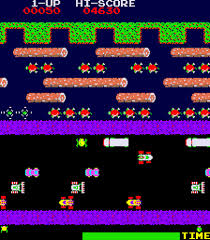
\includegraphics[width=6cm]{images/frogger.jpg}
    \caption{Cena do Jogo Frogger}
    \end{figure}


%%%%%%%%%%%%%%%%%%%%%%%%%%%%%%%%%%%%%%%%%%%%%%%%%%%%%%%%%%%%%%%%%%%%%%%%%%%%%%%%%%%%%
% Capítulo 4
% 
\chapter{Recursos da Linguagem}

\section{Orientação a objetos}

\begin{citacao}
Programação Orientada a Objetos (também conhecida pela sua sigla POO) é um modelo de análise, projeto e programação de software baseado na composição e interação entre diversas unidades chamadas de 'objetos'. \cite{wiki_oo}
\end{citacao}

\subsection{Classe Carro: Polimorfismo de sobrecarga, encapsulamento e herança}


 Especifica a altura (em coordenadas), largura, cor e coordenadas de surgimento dos carros no jogo, além disso especifica a movimentação e a velocidade do carro.É notado o polimorfismo de sobrecarga no caso de variáveis alternativas no método Move e o uso de getter and setter do atributo PositionY na def PositionY para o getter e setter PositionY\_  para o getter.Já notamos que um atributo sempre deve ter um valor inicial.
    
 Além disso a herança de um classe Java mostrando a interação da orientação a objetos Scala com Orientação a objetos Java,uma das principais caracteristicas da linguagem.

 Os getter e setters dos atributos da classe no construtor são feito de forma automática, porém caso queiramos um setter com lançamento de erro é possível produzir um na classe como vemos no atributo privado positionY de carro, onde ele manda uma exceção caso o valor do parâmetro do getter esteja dentro da área do rio do jogo.

 Além do encapsulamento private e public que é o padrão a outros modos de encapsulamento como:

\begin{enumerate}
    \item private[classe1] :  O atributo só é presente para a instância na classe1.
    \item protected : Atributo só presente nas classes filhas.
    \item private[pacote1]: O atributo só pode acessados em classes no pacote1.
\end{enumerate}

\newpage
Cógigo Scala da classe Car:
\begin{lstlisting}
package frogger.screen.`object`.Car
import javafx.scene.paint.Color
import javafx.scene.Node
import frogger.screen.`object`.Frog.RetangleObject

class Car(height:java.lang.Double , width: java.lang.Double , color: Color, MinSpawnY: java.lang.Double , MaxSpawnY:java.lang.Double ) extends RetangleObject {
    private var _PositionY: Double = 0.0
    
    def PositionY_=(value: Double): Unit = _PositionY = {
        if (value<335) {
            throw new ExceptionInInitializerError()
        }
        else {
            value
        }
    }
    
    def PositionY = _PositionY
    var right:Boolean=true;
    try
    {
        setGameObjectRectangle(height,width, color)
    }
    catch {
        case e:ExceptionInInitializerError => print("ERRO DE INICIALIZACAO")
    }
    var RandomPosition = math.random()
    private var Velo:java.lang.Double=0.0
    Velo=math.ceil(RandomPosition * (MaxSpawnY-MinSpawnY+1));
    
    if(math.ceil(RandomPosition * (MaxSpawnY-MinSpawnY+1))%2==0){
        right=true;
        try {
            PositionY = (0.1 * (math.ceil(RandomPosition * (MaxSpawnY - MinSpawnY + 1)) + (MinSpawnY - 1)) * 14) * 40
        }
        catch{
            case e:ExceptionInInitializerError => print("ERRO DE INICIALIZACAO D")
        }
        move(800, PositionY)
    }
    else{
        right=false
        try {
            PositionY = (0.1 * (math.ceil(RandomPosition * (MaxSpawnY - MinSpawnY + 1)) + (MinSpawnY - 1)) * 14) * 40
        }
        catch{
            case e:ExceptionInInitializerError => print("ERRO DE INICIALIZACAO D")
        }
        move(NodeX(), PositionY)
    }
    
    def move( ): Unit =
    {
        if(right) {
            move(NodeX() - 1 * Velo, NodeY())
        }
        else{
            move(NodeX() + 1 * Velo, NodeY())
        }
    }
}
\end{lstlisting}


\newpage
\subsection{Classe Frog e Polimorfismo de Inclusão e  Sobrecarga de Construtores}

Especifica altura, largura e cor do Sapo e verifica se ganhou (chegou do outro lado - coordenada Y <= 0) nos metodos. Da pra notar o polimorfismo de inclusão no método move modificado e  com \textit{override}.O polimorfismo de inclusão tem vinculação dinâmica igualmente a Java.

 Além de vários tipos de construtores fazendo polimorfismo de sobrecarga com construtores, nota-se isso nos métodos com this. Nota-se o construtor padrão no corpo da classe algo bastante útil para linguagem Scala deixando ela mais expressiva, isso é utilizado em quase todas classes do projeto orientado a objetos.
 
 Na classe lake do projeto pode se notar a definição de um operador da linguagem Scala como método.

 Além de vários tipos de construtores fazendo polimorfismo de sobrecarga com constructores. Nota-se o construtor padrão no início da classe algo bastante útil para linguagem Scala deixando ela mais expressiva e os getter And setter das variáveis são feitos de forma automática, como já citado.

\begin{lstlisting}
def +(that: Log) {
   logs=logs:::List(that)
 }
\end{lstlisting}

\newpage
Código Scala da classe Frog:

\begin{lstlisting}
    
    class Frog(var height:java.lang.Double ,var width: java.lang.Double ,var color: Color ) extends RetangleObject {
         try
         {
            setGameObjectRectangle(height,width, color)
         }
         catch {
            case e:ExceptionInInitializerError => print("ERRO DE INICIALIZACAO")
         }
         finally {
            setGameObjectRectangle(38.0,38.0, Color.GREEN)
         }
         
         def this(height:java.lang.Double, width:java.lang.Double ) = this(height, width, Color.GREEN);
         
         def this()=this(38.0,38.0,Color.GREEN);
         
         def CheckWin(): Boolean ={
            return (NodeY()<=0);
         }
            
         override def move(x: Double,y: Double): Unit ={
            if(y>600||x>=800||x<0){
            }   
            else{
                print(y);
                super.move(x,y);
            }
         }
    }
\end{lstlisting}


\newpage
\subsection{Classes Abstratas}

\begin{lstlisting}
 abstract class RetangleObject extends PositionObject {
   @throws(classOf[IllegalArgumentException])
    def setGameObjectRectangle( x: java.lang.Double, 
    y: java.lang.Double,  Color:Paint) {
         if(x<=0 || y<=0) 
         throw new 
         IllegalArgumentException("Only Positive Numbers")
          var  GameObjectRectangle :  Rectangle =
          new Rectangle(x, y, Color);
          setNode(GameObjectRectangle);
          return;
        }
    }
}
\end{lstlisting}

Aqui temos a definição da classe de todos os objetos retangulares no jogo. Classe herda uma classe Java e é abstrata, ou seja não pode haver objetos com essa Classe e é também abstrata.

Notamos no código o uso de tratamento de exceções para o caso de a formação de um Retangle com valores de diametro e altura negativa, lançando o IllegalArgumentException, também a herança da classe abstrata Java. Esse codigo representa um objeto retangular.

Na classe Abstrata RunningObject notamos os Getter and Setter da PositionY variavel que define a posição do objeto. Essa classe apresentada na página seguinte é dos objetos que correm na lagoa de forma determinística.

\newpage  
\begin{lstlisting}

abstract class RunningObject(height:java.lang.Double, width: java.lang.Double, color: Color, var _positionY: java.lang.Double, var right:java.lang.Boolean) extends RetangleObject {

  def move( Velo : java.lang.Double): Unit =
      {
        if(right) {
          super.move(NodeX() - 1 * Velo, NodeY())
        }
        else{
          super.move(NodeX() + 1 * Velo, NodeY())
        }
      }
  def positionY_= (value:Double):Unit = _positionY = value
  def positionY:Double = _positionY
} 
\end{lstlisting}

\newpage
\subsection{Sistema de exceções Scala}

 O sistema de tratamento exceções de Scala é muito parecido com o da linguagem Java, invés de lançar um valor novo, o programa lança uma classe de erro, os tratadores são ligados a trechos de códigos. Funções não precisam em si tratar exceção em todas as ocasiões. Assim pode ter classe que tem como herança exceções padrões da linguagem Java e Scala, ou seja todas exceções são classes e tem propriedades de orientação a objetos de acordo com suas características.

 No caso de erro não ser tratado o programa não executa fazendo o programa parar a execução na linha do erro. Todos os métodos e funções Scala podem lançar erros tendo lançamento de exceções e as exceções não precisam ser checadas no corpo da função, diferente de Java por exemplo, onde checar erros que serão lançados no corpo da classe é visto como um ponto negativo dessa linguagem por parte dos seus usuários. O corpo do tratamento de exceções usa try, catch e finally, como diversas linguagens modernas como Python com detecção de exceções.

 É possível usar \textit{pattern matching} para tratar os erros. Por não ser checado a exceção no método é possível criar uma lista de exceções para serem tratadas em todos os métodos de um programa, sem ser preciso declará los em todos os métodos. Um erro bem comum na linguagem Scala é de compatibilidade de algumas estruturas de dados de Java para Scala, esse é um elemento bem diferente de outras linguagens, mais populares que não tem compatibilidade entre si e as outras linguagens sem uso de bibliotecas externas. Scala não tem Exceções declaradas no contrato da classe, visto a enorme reclamação dessa pratica em outras linguagens de programação.

Segue um exemplo do uso de Try and Catch e lançamento de exceção no projeto:

\begin{lstlisting}
try
{
    setGameObjectRectangle(height,width, color)
}
catch {
    case e:ExceptionInInitializerError => print("ERRO DE INICIALIZACAO")
}
finally {
    setGameObjectRectangle(38.0,38.0, Color.GREEN)
}
\end{lstlisting}

Lançamento de Erro em uma função:
 
 \begin{lstlisting}
 def setGameObjectRectangle( x: java.lang.Double, y: java.lang.Double,  Color:Paint) {
    if(x<=0 || y<=0) throw new ExceptionInInitializerError()
     var  GameObjectRectangle :  Rectangle = new Rectangle(x, y, Color);
     setNode(GameObjectRectangle);
     return;
 }

\end{lstlisting}


\subsection{Destrutores e Coletor de Lixo de Scala}

 Não há destrutores em Scala, pois Scala tem Java Garbage Collections da Java Virtual Machine (JVM), que é algo já incluído no Kit de Desenvolvimento para a JVM. Os \textit{Garbage Collectors} executam o controle da memória de forma que o desenvolvedor não precisa se importar com isso no desenvolvimento. \cite{plumbr}
 
 É possível configurar o modo que o sistema de Coleta de Lixo funciona, mas essa configuração é de mínima necessidade na maioria dos projetos e é raramente usada. Isso porque a usada atualmente pelo Kit de desenvolvimento Java é a mais otimizada normalmente.

 O coletor de lixo usa uma Coleção de Gerações com diversos algoritmos, e estes podem variar dependendo da versão e da área do coletor de lixo Java.
    
\newpage   
\subsection{Classes Genéricas e Polimorfismo Paramétrico}

 As classes genéricas foram muito usadas em estruturas da Linguagem Scala segue a lista de exemplos em código de sua instancia e corpo da classe, que é o ID da classe \textit{gamescene}, T representa a classe abstrata:

\begin{lstlisting}
class IDOBJETO[T]() {
    private var _id: T = asInstanceOf[T]
    private var _idName:String =""
    
    def id = _id
    def id_= (newVal:T) = {
        _id = id
        try {
            idName=id.toString()
        }
        catch{
            case e:java.lang.Error=> print(e.getMessage)
        }
    }
    private def idName:String = _idName
    private def idName_=(newVal:String)={
        _id = id
    }
}
\end{lstlisting}

\begin{lstlisting}
var idscene:IDOBJETO[Int]= new IDOBJETO[Int]
idscene.id_=(1)
\end{lstlisting}
Definição de classe Genérica e logo depois sua instância acima.


\newpage
\subsection{Recursos não utilizados}

Os recursos não necessários no projeto foram as classes finais, pois se fosse um projeto continuo as classes teriam filhos. Também não foi utilizado Traits, que são usados para colocar propriedades de um objeto com o uso de funções que serão convertidos para métodos de um objeto que herda um Trait, o que é diferente de Interface, Interfaces não implementam a função, Traits são essenciais para herança múltipla em Scala, junto a definição de que método das classes pai usar com identificação de que classe usar o método, o que resolve o problema do diamante semelhante a solução de C++. É possível adicionar um Trait em um objeto com o uso de With.

   Exemplo de traits retirados do site oficial da linguagem Scala \cite{scala}
   \begin{lstlisting}
trait Iterator[A] {
    def hasNext: Boolean
    def next(): A
}

class IntIterator(to: Int) extends Iterator[Int] {
    private var current = 0
    override def hasNext: Boolean = current < to
    override def next(): Int =  {
        if (hasNext) {
            val t = current
            current += 1
            t
        } else 0
    }
}

val iterator = new IntIterator(10)
iterator.next()  // returns 0
iterator.next() 
   \end{lstlisting}
   
  Há também os Singleton Objects que são basicamente semelhantes Singletons de JAVA podendo armazenar classes únicas.
  
\subsection{Recursos não presentes em Scala}

 Não foi encontrado a possibilidade de Delegates nessa linguagem nem na linguagem Java. Uso de ponteiros também não, somente na leitura de arquivos. 
  

\section{Programação Funcional}

Scala com certeza é muito melhor com auxílio de Java para linguagem Funcional, o que dificulta a utilização de artifícios puramente funcionais no desenvolvimento, principalmente por causa do uso de bibliotecas Java.

 O projeto utilizou Java somente para lidar com a biblioteca gráfica JavaFX e com a questão da comunicação entre Scala Funcional e Java, o que se notou um aspecto bem positivo na linguagem, embora atualmente Java já tenha muitos recursos das linguagens funcionais.

\subsection{Currying, Map e Funções imutáveis e pattern matching}

Em Scala é possível aplicar muitos dos conceitos de programação funcional em poucas linhas de código, como temos abaixo:
\begin{lstlisting}
    def Movecars(nodes: java.util.List[Rectangle], move:java.lang.Double):java.util.List[java.lang.Double] = {
            getX(nodes).map((x:Double)=> x match{
                case 100000 => 100000
                case x1 if x1>800||x1<0 => 100000
                case _ => x + move
            }).map(Double.box).asJava
        }
\end{lstlisting}

  Essa função retorna a coordenada X em Double para todos os carros somada a movimentação de carro, junto a função de volta ao ponto inicial de um carro que saiu da tela para poder ser renascido futuramente. Podemos notar primeiro na função MoveCars o uso da função GetX que uso map para retornar o valor X de todos Nodos, usando uma função Java, assim possível de programar em com métodos Java em Scala funcional.

   Logo após isso vemos mais uma característica das linguagens funcionais, o uso de currying, primeiro passamos a função anônima, e disso se gera a função que dado esse move calcula a possibilidade de desaparecimento na tela de um carro ou da sua movimentação com o uso de map novamente. Também é interessante pelo uso de \textit{Pattern Matching}.


\subsection{Funções de alta ordem com métodos Java   e Recursão como Iteração}
\begin{lstlisting}
var SpawnCars:(List[Rectangle], List[Double=>Unit]) => (Double=>Unit) = (cars: List[Rectangle], ChangeFunction:List[Double=>Unit])
=> cars match {
        case Nil => (x: Double) =>
        case _ => cars.head.getTranslateX match {
        case 10000=> ChangeFunction.head
        case x1 if x1>800||x1<0 => ChangeFunction.head
        case _ => cars.isEmpty || ChangeFunction.isEmpty match {
        case true => (x: Double) =>
        case false => SpawnCars(cars.tail, ChangeFunction.tail)
     }
   }
 }
 
\end{lstlisting}

Nessa função nota-se o uso de recursão como método de iteração dado uma lista de retângulos, os carros do jogo e uma lista de funções, as funções de movimentação de cada carro, é possível retornar uma função que move o carro que vai renascer na Tela.

Assim se notando duas características das funções da Alta Ordem, função como parâmetro e retorno de função como saída de funções.

\newpage
\subsection{Outros recursos funcionais usados e variaveis anonimas não declaradas}
Uso de Reduce e variáveis Anônimas sem declaração, é notório também uso de variáveis anônimas sem declaração na seção de processamento paralelo em Scala Funcional.

Elementos de primeira ordem são notórios quando se declara funções como variável e se passa uma função como parâmetro como se nota quando é passado uma lista de função como parâmetro na função SpawnCars.



\begin{lstlisting}
var FrogDeath:( Node, Rectangle, List[Rectangle], List[Rectangle], List[Rectangle], Double, Double, Boolean) => java.lang.Double= (frog: Node, Lake: Rectangle, Logs: List[Rectangle], carsR: List[Rectangle], carsL: List[Rectangle], restart: Double, atual: Double,carContact:Boolean) =>
 frog.getTranslateY  match {
   case y if y < 161 => y
   case _ => CheckLake(frog, Lake) match {
     case true => !(Logs.map((item: Rectangle) => item.getBoundsInParent.intersects(frog.getBoundsInParent) ).reduce( _ || _ )) match {
        case true => restart
        case false => atual
     }
     case false=> carContact match {
        case true => restart
        case false =>carContact match{
            case true=>restart
            case false =>atual
       }
     }
   }
 }
\end{lstlisting}


\newpage
\section{Processamento Paralelo}

Para melhorar o desempenho e de acordo com os requisitos para este projeto, utilizamos a programação paralela.

\subsection{Orientação a Objetos}
 Durante o desenvolvimento do projeto com orientação a objetos se utilizou as classes de Thread Java para mostrar ser possível a interação de multiparadigma Java e linguagem sem Pacote para criação de programação paralela com o uso de Classes. Porém é possível também instanciar classes Scala com herança da classe Thread Java.
 
\begin{lstlisting}
class Task1 extends Thread {
   public gamescene gamescene1;
   public List<Car> cars;

   Task1(gamescene g, List<Car> car) {
       this.gamescene1 = g;
       this.cars = car;
   }

   @Override
    public synchronized  void run() {
       gamescene1.SpawnCars();
   }
}

class Task2 extends Thread {
   public gamescene gamescene1;

   Task2(gamescene g) {
       this.gamescene1 = g;
   }

   @Override
   public  void run() {
       gamescene1.movelogs(10.0);
   }
}
\end{lstlisting}


Abaixo o código para criar objetos da classe  \textit{Thread} e executa-las.
\begin{lstlisting}
Task1 task1 = new Task1(gamescene1, cars);
Task1 task3 = new Task1(gamescene1, cars);
Task2 task2 = new Task2(gamescene1);
task1.run();
task3.run();
task2.run();
\end{lstlisting}

O processamento da \textit{Threads} da classe Thread Java é assíncrono e síncrono no projeto, é possível sincronizar para não ocorrer condição de corrida que atrapalhe com a modificação de regiões críticas de forma a dar um resultado inesperado.
\newpage

\subsection{Programação Funcional}
A programação paralela em paradigma funcional é onde a linguagem Scala brilha na sua independência da linguagem Java. O principal método é o uso de \textit{Future} e \textit{Promise} foi feito tendo em mente a linguagem Funcional e é assíncrono \cite{wiki_future},por ser imutável logo quando declarada é muito boa para o paradigma funcional,podendo  e foi criada graças ao paradigma funcional e logo se veio em uso em paradigmas semelhantes como o lógico.

 Sua principal característica é o uso de future uma função que ser executada em outra thread de forma imutável,tendo 3 estados um Future:
  \begin{enumerate}
\item Completo,sem exceções
\item Completo ,com exceções
\item Incompleto
 \end{enumerate}

 O tipo de dado Promise serve para fazer comunicação entre Futures segue o exemplo do código no site oficial da linguagem:
\begin{lstlisting}
import scala.concurrent.{ Future, Promise }

val p = Promise[T]()
val f = p.future

val producer = Future {
 val r = produceSomething()
 p success r
 continueDoingSomethingUnrelated()
}

val consumer = Future {
 startDoingSomething()
 f onSuccess {
   case r => doSomethingWithResult()
 }
}
\end{lstlisting}

 "P sucess r” faz com que o future consumer execute a função doSomethingwithResult() caso seja completo sem exceções a atribuição da variável r na função anônima producer. 
  
 Exemplo de uso de código com Future no projeto com uso de método Await, bastante útil para execução paralela, que tem como segundo parâmetro o tempo máximo de espera para o future ser terminado, abaixo a chamada de dois futures, para achar o contato de carros com o sapo no Frogger.
 
 \begin{lstlisting}
def frogDeath(frog: Node, Lake: Rectangle, LogR:Rectangle,LogL:Rectangle,LogLL:Rectangle, carsR: java.util.List[Rectangle], carsL: java.util.List[Rectangle], restart: java.lang.Double, atual: java.lang.Double) = {
    
    var carL = carsSIDEContact(frog,carsR.asScala.toList,Lake)
    var carR = carsSIDEContactR(frog,carsL.asScala.toList,Lake,carL)
    
    FrogDeath(frog, Lake, List(LogR,LogL,LogLL), carsR.asScala.toList,carsL.asScala.toList, restart, atual,Await.result(carR,100 seconds))
}
\end{lstlisting}

Abaixo a definição dos futures do tipo Boolean:

\lstset{style = MyJava}
\begin{lstlisting}
val carsSIDEContact=(frog:Node,cars: List[Rectangle],Lake:Rectangle)=>{
 Future[Boolean] {
   CheckLake(frog, Lake) match {
     case true => true
     case false => cars.map((item: Rectangle) => item.getBoundsInParent.intersects(frog.getBoundsInParent) ).reduce(_ || _)
   }
 }
}
var carsSIDEContactR=(frog:Node,cars: List[Rectangle],Lake:Rectangle,future2:Future[Boolean])=>{
 Future[Boolean] {
   CheckLake (frog, Lake) match {
     case true => true
     case false => cars.map ((item: Rectangle) => item.getBoundsInParent.intersects(frog.getBoundsInParent) ).reduce (_ || _ ) match{
       case true=>true
       case false=>Await.result(future2,100 seconds)
     }
   }
 }
}
 \end{lstlisting}
 
 \subsection{Extra}
 Existem outros modelos de programação paralelas na linguagem Java como a biblioteca externa Java e Scala Akka \cite{akka}, não usadas neste projeto. Ela usa um modelo diferente de programação paralela comparada as vistas anteriores, usa o modelo \textit{Actor Model}.

 Há inúmeras outras maneiras de se utilizar programação paralela devido a quantidade absurda de bibliotecas Java de processamento Paralelo.

%%%%%%%%%%%%%%%%%%%%%%%%%%%%%%%%%%%%%%%%%%%%%%%%%%%%%%%%%%%%%%%%%
\chapter{Análise Crítica}

\begin{longtable}[c]{|p{4cm}|c|p{8.8cm}|}
\caption{Análise Crítica}
\hline

\textbf{Propriedades} & \textbf{Nota} & \textbf{Observações} \\ \hline
\endfirsthead
\multicolumn{3}{c}
{\tablename\ \thetable\ -- \textit{Continuação da Pagina Anterior}} \\
\hline
\textbf{Propriedades} & \textbf{Nota} & \textbf{Observa\c{c}oes} \\ \hline
\endhead
\hline \multicolumn{3}{r}{\textit{Continua na próxima pagina}} \\
\endfoot
\hline
\endlastfoot

custo                           & 7 & Devido a sua comunidade reduzida existe poucos materiais de boa qualidade, principalmente em video, o que dificultaria a resolução de problemas em sites como Stackoverflow e aumentaria os custos de um treinamento da linguagem. A IDE recomendada pelo site oficial de Scala IntelliJ IDEA (que é uma IDE proprietária e portanto também tem um custo) facilitou a compilação, mas teve diversos projetos para fazer as configurações dessa compilação. Seu aprendizado acaba por ser mais fácil para desenvolvedores que já são familiarizados com a linguagem Java por suas similaridades. Seu tempo de compilação é mais baixo que Java e Go.
O código da linguagem Scala é totalmente de código aberto, o que ajuda na facilidade e confiabilidade.
\\\hline
eficiência                      & 7 & Linguagem bastante eficiente em questão de tempo de execução em comparação a outras linguagens do ambiente virtual Java, até mais rápido que Java como mostra o artigo do Google \cite{lricjgs}, porem mais devagar no tempo de execução do que linguagens como Go e C++, que são compiladas e não interpretadas. Alto custo de memoria muito parecido com Java, o alto custo de memoria de aplicações do ambiente virtual Java já é algo de muito conhecimento dos programadores dessas linguagens.
\\\hline
generalidade                    & 10 & Sendo uma linguagem de propósitos gerais Scala consegue se sair muito bem em um grande número de aplicações principalmente voltadas ao alto nível (visto que é uma linguagem interpretada), no nosso trabalho desenvolvemos um jogo mas não acho que teríamos problema para desenvolver um sistema para uma loja usando a mesma linguagem. 
\\\hline %%%%talvez retirar esse último trecho. revisitar logo.
simplicidade                    & 7 & Como uma linguagem parecida com Java mas um pouco mais compacta \cite{matt}, ela tem simplicidade em comparação as outras linguagens pois não requer que para um projeto pequeno seja necessário adornos. 
\\\hline
portabilidade                   & 10 & Compilado para Maquina Virtual Java  feita pela oracle, suportada em diversas plataformas com .Net e com compatibilidade de fácil implementação, pode ser usado no sistema operacional Android, maior sistema para Celulares, compatível em programação de interfaces web por meio de Scala.js, Scala é sem dúvida uma mão cheia no sentido de portabilidade.
 \\\hline
reusabilidade                   & 8 & Apresenta uma boa reusabilidade por ter suporte a classes, polimorfismo universal com mecanismos de herança e suporte a tipos genéricos.  
\\\hline
ortogonalidade                  & 7 & Relacionada a legibilidade e simplicidade, Scala consegue ter uma boa relação com tais e faz uso tranquilo de combinações com segurança. 
\\\hline
expressividade                  & 10 &  Scala é uma linguagem focada na expressividade,``Scala faz coisas simples serem fáceis e coisas difíceis serem possiveis`` é um dos \textit{mottos} que achamos na internet ao pesquisar sobre a linguagem principalmente ao se tratar do paradigma funcional. 
\\\hline
modelo de tipos                 & 9 & Conta com uma verificação de tipos estática e dinâmica. Variáveis em Scala não necessitam de declaração por tipo (declaração usando \textit{var} porém se preferirmos otimizar podemos definir por tipos como int e float) contém polimorfismo por coerção tipos menores são convertidos para tipos maiores, mas o contrário não é válido.
\\\hline
tamanho de código               & 7 & Não consegue ser menor o tamanho de codigo do que a maioria das linguagens Scripts por ter que definir os tipos em alguns casos,caso se use Java junto com Scala o tamanho do codigo aumenta muito porém o uso de somente linguagem Scala se vê usar menos codigo que linguagens modernas compiladas como Go,pode se notar isso no artigo do Google já citado. \\\hline
suporte e documentação          & 8 & A documentação padrão do site da Scala é muito boa e bem completa e também conseguimos achar tutoriais sobre os mais diversos temas em sites diferentes pela internet envolvendo Scala, porém comparada a linguagens mais \textit{mainstream} como C++ ou Java temos um número reduzido de vídeos tutoriais e exemplos de código.
\\\hline
suporte a abstração de dados 
e de processos                  & 8 & Scala possui um ótimo suporte a abstração principalmente de dados, o que facilita para quem já possua experiência com a linguagem fazer o que quiser.
\\\hline
adequabilidade e variedade 
de estruturas de controle       & 7 & Scala possui uma relação comum com o que a maioria das linguagens apresenta com esse quesito, possui as estruturas mais comuns mas tem seus detalhes para serem bem utilizadas em todos os paradigmas.
\\\hline

\end{longtable}

\section{Porque Orientação a Objetos é melhor}

  Visto que a maioria das bibliotecas usadas no desenvolvimento com linguagem Scala são na verdade bibliotecas feitas em Java e utilizadas por compatibilidade, é quase inviável não se usar a Orientação a Objetos com as melhores Bibliotecas da linguagem Scala que são de Java, uma linguagem totalmente baseada na orientação a objetos e que apenas recentemente ganhou a habilidade de usar recursos funcionais como \textit{currying}, mesmo assim suas bibliotecas não foram feitas pensando no uso de paradigma funcional puro.


%%%%%%%%%%%%%%%%%%%%%%%%
\chapter{Melhoramentos}

\section{Interação Java}
 A interação entre Java e Scala poderia ser melhor por exemplo, poderia ser possível decidir previamente que todas as estruturas do módulo java que são semelhantes ao módulo Scala tenham tradução direta para Scala caso passe algum parâmetro para função Scala ou Java, esse argumento seja passado de Java para Scala ou vice versa de maneira que isso seja implementado de forma automática, claro o usuário pode mudar isso da maneira que preferir o desenvolvimento, também pode fazer traduções de estruturas Java e Scala de forma automática. Poderia ser possível que o ambiente de desenvolvimento faça isso, mas se a linguagem fizesse isso de fato seria muito melhor.

\section{Dependência Java}
 Por Scala ser uma linguagem interpretada pela Java Virtual Machine é difícil ver algum projeto de grande porte que não interaja com a linguagem Java ou com suas estruturas.

 Bibliotecas que só usam Scala podem torná-la uma linguagem independente, sentimos que que há certa dificuldade no uso do paradigma puro funcional pois de uma forma ou outra acabamos tendo que recorrer eventualmente a orientação a objetos presente no Java em suas bibliotecas. Por outro lado o uso dessa abordagem aparentemente tem se tornado cada vez mais comum visto que a maioria das linguagens modernas de propósito geral já são multi-paradigma (ex: C++, C\#, Python), então é de se esperar que Scala use suas funcionalidades de forma intercalada \cite{stack}.

\section{Comunidade}

 A comunidade de Scala ainda não é tão forte, é difícil achar bibliotecas feitas especificamente para a linguagem Scala, como já citado, e tutoriais e documentações dessas bibliotecas, assim como tutoriais de conceitos básicos, faltam exemplos de codificação em Scala na internet.

 Ainda sobre a falta de comunidade é notório a falta de vídeos e tutoriais de uso de bibliotecas e a Linguagem, um bom exemplo é a falta de códigos exemplo da biblioteca ScalaFx no seu site oficial. A equipe de desenvolvedores poderia colocar exemplos de cada classe como faz a equipe da JavaFX, o que facilitaria muito mais o aprendizado e com isso faria os desenvolvedores priorizarem o uso de uma biblioteca da própria linguagem ao invés de escolher uma da linguagem Java que seja compatível, mesmo que ao custo de ter que trabalhar com a conversão de alguma classe Java para uma semelhante em Scala.

 Uma solução seria adicionar a compatibilidade de Scala a pacotes multi linguagens, como as que utilizem \textit{wrapped library} para compatibilidade. Notórios pacotes que funcionam em diversas linguagens OpenMP e no caso a que é utilizada pelo grupo de neurociência computacional da UFRGS labstreaminglayer. Outra solução é a defesa do uso de linguagem Scala para aprendizado de crianças e iniciantes em programação, como é notório ver isso como um dos motivos pelo crescimento da linguagem Ruby e Python.

%%%%%%%%%%%%%%%%%%%%%%%%%%%%%%%%%%%%%%%%%%%
\chapter{Scala e Desenvolvimento de Jogos}

 A linguagem Scala não é a mais indicada para desenvolvimento de Jogos, principalmente pela sua não compatibilidade com Engines Gráficas de renome como Unity e Godot. Apesar de ter boas bibliotecas gráficas 2D em Scala, todas as mais conhecidas requerem conhecimento de Java ou no mínimo das classes da linguagem Java.
 
  Além disso, o processamento paralelo em Scala é pouco intuitivo, o que dificulta aprender esse recurso tão importante para o desenvolvimento de jogos. O desenvolvimento do jogo Frogger foi bem trabalhoso, mas a produção do jogo usando os dois recursos foi viável.

\chapter{Conclusão Geral}

Scala é uma boa linguagem, mas não é recomendável se o usuário não tiver conhecimento ou interesse em classes de Java, pois se estiver focando em produtividade será obrigado a usar a linguagem Java e ter conhecimento sobre suas classes e frameworks. A curva de aprendizado é complicada devido a uma certa escassez de material online (além da documentação padrão) e conta com um número de usuários relativamente pequeno em relação a outras linguagens estudadas anteriormente no nosso curso.

A interação entre Java e Scala é por vezes problemática, mas não deixa de ser um ponto muito positivo da linguagem essa possibilidade de integração. A necessidade de poucas linhas de código para programas relativamente complexos em Scala é um dos seus principais pontos positivos, principalmente quando se trata do paradigma funcional, é também muito bom usar map em Scala para métodos de Java. Um possível problema para Scala é que a linguagem Java está adicionando cada vez mais recursos funcionais, o que pode tornar o aprendizado de Scala, para uso do paradigma funcional no código Java (um dos principais motivos do crescimento de sua comunidade), inútil. 

A escolha foi interessante pelo aprendizado de diversos conceitos como Java Virtual Machine, conceitos de Paradigma funcional e novos modelos de programação paralela com Future e Promisse.

Uma das principais dificuldades encontradas no Desenvolvimento do Jogo Frogger foi a compilação do código em Scala, utilizamos a IDE IntelliJ que é recomendada no próprio site da linguagem, o ambiente de desenvolvimento realmente facilitou a compilação organizando a estrutura dos arquivos para a compilação certa, porém houveram alguns problemas, principalmente na primeira compilação (nos dois paradigmas) e no processo de configurar o Kit de desenvolvimento Java na IDE\cite{intellij}.

%%%%%%%%%%%%%%%%%%%%%%%%%%%%%%%%%%%%%%%%%%%%%%%%%%%%%%%%%%%%%%%%%%%%
% Referências 

%\bibliographystyle{abnt}

\bibliographystyle{abntex2-alf}

\bibliography{biblio} % arquivo que contém as referências (no formato bib). Colocar as suas lá (se tiver dúvida sobre como adicionar novas referências, usar o software JabRef ou Medley)

\end{document}